\section{Methodology}
\label{sec:methodology}

\subsection{Embedding models}

I undertook this task to investigate the relative performance of pre-trained static and
contextual embeddings for a context-dependent word-similarity task.
To this end, Transformer models \parencite{Vaswani2017} were a natural choice.
The baseline models for the task were the multilingual BERT model
\parencite{Devlin2019} and ELMo models \parencite{Peters2018a} trained on Finnish,
Croatian, and Slovene datasets \parencite{Ulcar2020a}; and the vast majority of the
task submissions used Transformers \parencite[36,42-45]{Armendariz2020a}.
The models that I evaluated were accessed via the HuggingFace \emph{Transformers}
library \parencite{Wolf2020} and are listed in \cref{table:language-models}.

\begin{figure}
  \centering
  \begin{tabular}{lcccc}
    Model name                                                        & English    & Finnish    & Croatian   & Slovene
    \\
    \hline
    \texttt{EMBEDDIA/crosloengual-bert}\textsuperscript{1}            & \checkmark & \checkmark &
    \checkmark                                                        & \checkmark
    \\
    \texttt{TurkuNLP/bert-base-finnish-cased-v1}\textsuperscript{2}   &            & \checkmark &            &
    \\
    \texttt{TurkuNLP/bert-base-finnish-uncased-v1}\textsuperscript{2} &            & \checkmark &            &
    \\
    \texttt{TurkuNLP/bert-large-finnish-cased-v1}\textsuperscript{2}  &            & \checkmark &            &
    \\
    \texttt{bert-base-cased}                                          & \checkmark &            &            &
    \\
    \texttt{bert-base-multilingual-cased}                             &
    \checkmark                                                        & \checkmark & \checkmark & \checkmark
    \\
    \texttt{bert-base-multilingual-uncased}                           & \checkmark & \checkmark & \checkmark &
    \checkmark
    \\
    \texttt{bert-base-uncased}                                        & \checkmark &            &            &
    \\
    \texttt{bert-large-cased}                                         & \checkmark &            &            &
    \\
    \texttt{bert-large-cased-whole-word-masking}                      & \checkmark &            &            &
    \\
    \texttt{bert-large-uncased}                                       & \checkmark &            &            &
    \\
    \texttt{bert-large-uncased-whole-word-masking}                    & \checkmark &            &            &
    \\
    \texttt{classla-bcms-bertic}\textsuperscript{3}                   &            &            & \checkmark &
  \end{tabular}
  \caption{The pre-trained models from the HuggingFace \emph{Transformers} library
    \parencite{Wolf2020} that I evaluated for each language.
    The corresponding references are \textsuperscript{1}\textcite{Ulcar2020},
    \textsuperscript{2}\textcite{Virtanen2019}, \textsuperscript{3}\textcite{Ljubesic2021},
    and \textcite{Devlin2019} otherwise.
  }
  \label{table:language-models}
\end{figure}

The primary comparison that I made was between these models' static input and
contextual output representations.
Several of the submissions used a combination of a Transformer's hidden-states
\parencites[e.g.,][276]{Gamallo2020}[3]{Pessutto2020}[4]{Hettiarachchi2021}.
This choice is supported by the analysis of \textcite{Ethayarajh2019}, who found that
the upper layers of Transformer models produce more context-dependent representations.
Hence, I also evaluated an example of this approach—a thorough comparison of the
performance of its variants is, however, beyond the scope of this paper.
Hereafter, I refer to the three types of embeddings that I evaluated as:
\begin{itemize}
  \item \texttt{static}, the model's input embeddings;
  \item \texttt{contextual}, the model's output embeddings; and
  \item \texttt{pooled}, the sum of the model's last four hidden-states.
\end{itemize}

I note that I did not directly reproduce the baseline model because it requires the
\texttt{bert-embedding} Python package, which is incompatible with Apple's ARM-based
processors and has been deprecated since 2020 \parencite{Lai2023}.
However, the baseline is notionally equivalent to the \texttt{contextual} embeddings of
the \texttt{bert-base-multilingual-cased} model with a window size of zero.

\subsection{Composition operations}

The basic procedure that I employed is described in \cref{chart:schematic-procedure}.
For each pair of target words and each of the two contexts in which they appear, I
obtained a contextualised representation of a target word by: finding the index of the
target word's first sub-word token within the tokens of the target word's context;
finding the tokens within a fixed-size window around the target word's first token;
obtaining the embeddings of the tokens in the window; and combining the the embeddings
to produce a single representation of the target word.
Notably, the use of a sub-word vocabulary by the models in question
\parencite[e.g.,][4174]{Devlin2019} dictates that a target word may be represented by a
different number of tokens in each context.
As a result, the representations of a pair of target words may be different in each
context, even if they are static and the window size is zero.
This is the cause of the non-zero scores obtained by models of this kind, particularly
for the Finnish language (\cref{chart:score-window-static}).

\begin{figure}
  \centering
  \newcommand{\period}{\text{.}}
  \newcommand*{\orawidest}{accept}
  \newcommand*{\oratallest}{\#\#}
  \newlength{\orawidth}
  \settowidth{\orawidth}{\orawidest}
  \newcommand*{\ora}[1]{\overrightarrow{#1\vphantom{\oratallest}}}
  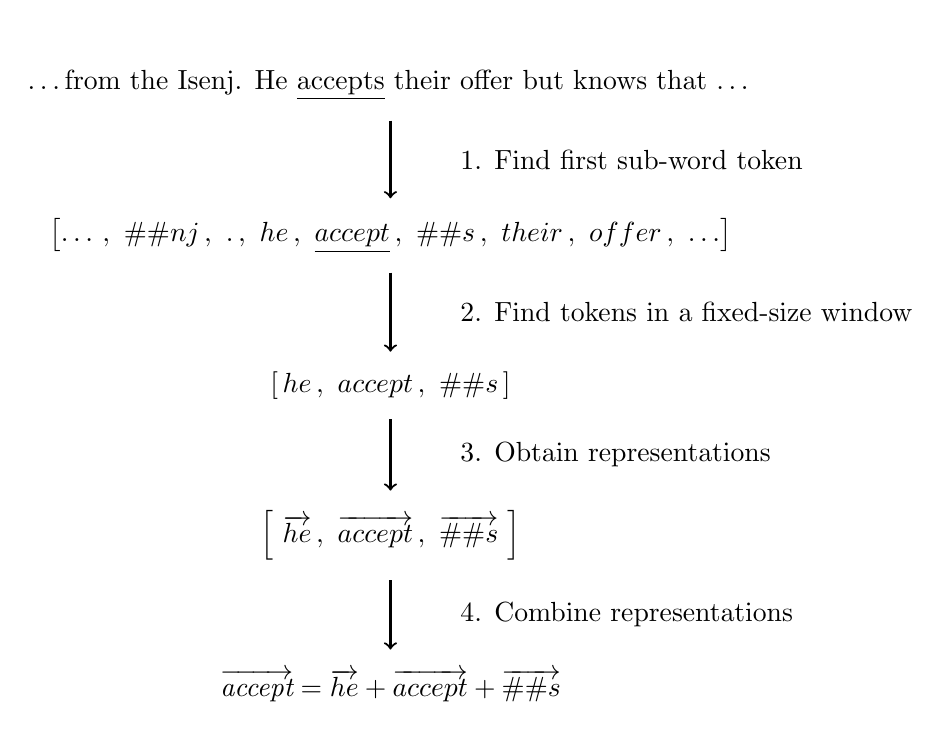
\begin{tikzpicture}[
      node distance = 0.75in,
      every node/.style = {
          inner sep = 0,
          outer sep = 0.1in
        }
    ]
    \node [label] (a) {
      \dots from the Isenj\period{}
      He \underline{accepts} their offer but knows that \dots }; \node [label, below of=a]
    (b) {$\left[ \dots\,,\ \text{\#\#nj}\,,\ \period{}\,,\ \text{he}\,,\
          \text{\underline{accept}}\,,\ \text{\#\#s}\,,\ \text{their}\,,\ \text{offer}\,,\ \dots
          \right]$}; \node [label, below of=b] (c) {$\left[ \, \text{he}\,,\ \text{accept}\,,\
          \text{\#\#s} \, \right]$}; \node [label, below of=c] (d) {$\left[ \ \ora{\text{he}}\,,\
          \ora{\text{accept}}\,,\ \ora{\text{\#\#s}} \ \right]$}; \node [label, below of=d] (e)
    {$ \ora{\textit{accept}} = \ora{\text{he}} + \ora{\text{accept}} + \ora{\text{\#\#s}}
      $}; \draw [thick, ->] (a) -- (b) node[midway, right=0.25in] {1.
      Find first sub-word token}; \draw [thick, ->] (b) -- (c) node[midway, right=0.25in] {2.
      Find tokens in a fixed-size window}; \draw [thick, ->] (c) -- (d) node[midway,
      right=0.25in] {3.
      Obtain representations}; \draw [thick, ->] (d) -- (e) node[midway, right=0.25in] {4.
      Combine representations};
  \end{tikzpicture}
  \caption{A schematic of the procedure used
    to obtain a contextualised representation of a target word from pre-trained embeddings.
    In this example, the target word is ``accept'', the window size is one (either side of
    the target word), and the composition operation is addition.
  }
  \label{chart:schematic-procedure}
\end{figure}

Inspired by \textcite{Landauer1997}, \textcite{Kintsch2001}, and
\textcite{Mitchell2008}, I predominantly investigated the application of element-wise
addition and multiplication as composition operations.
However, preliminary experiments indicated that multiplication performed poorly across
all languages, models, and window sizes; hence, it was discarded before the final
analysis.
Additionally, I chose to evaluate the concatenation (`stacking') of embeddings.
In the case that the number of embeddings was fewer than that expected for the window
size, i.e., the target word was close to the beginning or the end of its context, I
right-padded the concatenated embedding with zeros to obtain contextual embeddings of
equal length.
This approach was also inferior to addition for practically all combinations of
parameters.

\subsection{Window size}

Due to the computational expense of exhaustively searching the possible window sizes, I
applied heuristics to constrain the search space.
A naïve estimation of the average number of words in each context, i.e., segmenting on
whitespace, gave a result of between $40$ and $60$ for the different languages.
Therefore, for the static-embedding models, I chose $50$ as an upper bound on the
window size on either side of the target word.
The motivation to choose a smaller maximum window size for contextual-embedding models
was similarly economical (\cref{sec:cost-benefit}); however, as the window size
approaches the length of the sequence, one would expect a combination of token
representations to be superseded by the sequence-level representation of the model,
e.g., the special \texttt{CLS} token of BERT variants \parencite[4174]{Devlin2019}.
These heuristics were largely vindicated by the results of the evaluation, which
demonstrated that the scores decrease as the window size approaches the maximum.
